%! Author = spruhs
%! Date = 25.02.25

% Preamble
\documentclass[11pt]{article}

% Packages
\usepackage[utf8]{inputenc}
\usepackage[T1]{fontenc}
\usepackage[ngerman]{babel}
\usepackage{graphicx}
\usepackage{tocloft}
\usepackage{appendix}
\usepackage{csquotes}
\usepackage[
    backend=biber,
    style=alphabetic,
]{biblatex}
\usepackage{color}
\addbibresource{literaturverzeichnis.bib}

% Document
\begin{document}

    \begin{titlepage}
        \centering
        {\scshape\LARGE Seminar 1908 Moderne Programmiertechniken und -Methoden -Sommer 2025 \par}
        \vspace{1cm}
        {\huge\bfseries Kotlin statt Java\par}
        \vspace{1.5cm}
        {\scshape\Large Fabian Spruhs\par}
        {\scshape fabian@spruhs.com\par}
        \vspace{2cm}
        {\Large\itshape Studiengang Bachelor Informatik\par}
        \vspace{2cm}


        {\large \today\par}
    \end{titlepage}

    \tableofcontents
    \newpage


    \section{Einleitung}


    \section{Kurzvorstellung Java}

    \subsection{Übersicht}
    \begin{itemize}
        \item \textbf{Erscheinungsjahr:} 1995
        \item \textbf{Entwickler:} Sun Microsystems
        \item \textbf{Entwickler ab 2009:} Oracle Corporation
        \item \textbf{Programier paradigmen:} objektorientiert
        \item \textbf{Aktuelle LTS version:} 21
    \end{itemize}

    \subsection{Technischer Hintergrund}
    Java ist eine Programmiersprache, die von Sun Microsystems entwickelt und im Jahr 1995 veröffentlicht wurde.
    Sie zeichnet sich durch ihre Plattformunabhängigkeit, hohe Robustheit und vielseitigen Einsatzmöglichkeiten aus,
    wodurch sie insbesondere in der Industrie und im Unternehmensumfeld eine zentrale Rolle spieltS.

    Ein wesentliches Merkmal von Java ist die Art der Code-Ausführung.
    Anstatt direkt in Maschinencode übersetzt zu werden, wird der Quellcode
    zunächst in Bytecode kompiliert. Dieser Bytecode wird anschließend von
    der Java Virtual Machine (JVM) interpretiert und ausgeführt. Durch dieses
    Konzept ist Java nicht an eine spezifische Prozessorarchitektur oder ein
    bestimmtes Betriebssystem gebunden, was eine hohe Portabilität gewährleistet.
    Diese Plattformunabhängigkeit stellt einen bedeutenden Vorteil dar, den
    viele andere Programmiersprachen im Laufe der Zeit übernommen haben.

    Neben der Plattformunabhängigkeit bietet die JVM zahlreiche zusätzliche
    Funktionen, die zur Stabilität und Sicherheit von Java-Anwendungen
    beitragen. Dazu gehören unter anderem eine automatische Speicherverwaltung
    durch den Garbage Collector, eine starke Typisierung zur Minimierung
    von Laufzeitfehlern sowie eine integrierte Unterstützung für Multithreading,
    die eine effiziente nebenläufige Verarbeitung ermöglicht. \cite[51 - 54]{insel}

    Java basiert konsequent auf dem objektorientierten Programmierparadigma, das die Strukturierung von Software in Klassen und Objekte ermöglicht. \\

    \subsection{Verbreitung}
    Der TIOBE-Index misst monatlich die Popularität und Verbreitung von Programmiersprachen \cite{tiobe}.
    Laut diesem Index zählt Java zu den am weitesten verbreiteten Programmiersprachen weltweit.
    Wie in Abbildung \ref{fig:entwicklung-tiobe} ersichtlich, befand sich Java über fast zwei Jahrzehnte hinweg
    kontinuierlich unter den Top 3 der relevantesten Programmiersprachen.

    In den letzten Jahren hat die Popularität von Java zwar leicht nachgelassen, dennoch bleibt die Sprache weiterhin
    von großer Bedeutung. Auch im Februar 2025 belegte Java den dritten Platz im TIOBE-Index
    (siehe Abbildung \ref{fig:tiobe-java-2025}).

    Java ist die Basis zahlreicher Anwendungen und wird in vielfältigen Bereichen eingesetzt. Darüber hinaus
    verfügt Java über eine umfangreiche Ökosystemlandschaft mit einer Vielzahl an Bibliotheken, Paketen,
    Frameworks und Fachliteratur.

    Die weltweite Java-Community ist äußerst aktiv und umfasst eine große Anzahl an erfahrenen Entwicklern,
    die kontinuierlich zum Wissenstransfer und zur Weiterentwicklung der Sprache beitragen. Ein Beispiel für die
    Größe dieser Infrastruktur ist das Maven-Repository, das über 2.800 Repositories mit mehr als 52 Millionen Java-Paketen
    enthält \cite{maven}.

    Diese etablierte und breit aufgestellte Infrastruktur stellt einen weiteren entscheidenden Vorteil von Java dar und
    trägt zu seiner anhaltenden Relevanz in der Softwareentwicklung bei.\\


    \section{Kurzvorstellung kotlin}

    \subsection{Übersicht}
    \begin{itemize}
        \item \textbf{Erscheinungsjahr:} 2011
        \item \textbf{Entwickler:} Jetbrains
        \item \textbf{Programier paradigmen:} objektorientiert, funktional
        \item \textbf{Aktuelle LTS version:} 2.1.0
    \end{itemize}

    \subsection{Technischer Hintergrund}
    Kotlin wurde 2011 von der Firma JetBrains veröffentlicht. Ziel der Entwicklung war es, eine verbesserte Alternative zu Java zu schaffen.
    Schon an der Namensgebung kann man die nähe zu Java erkennen. Der Name Java bezieht sich auf eine Indonesiche Insel.
    Der Namensgeber von Kotlin ist eine russische Insel vor St. Petersburg.

    Obwohl Java nur etwa 15 Jahre älter als Kotlin ist, stellt dies in der schnelllebigen Welt der Softwareentwicklung eine erhebliche Zeitspanne dar.
    In vielerlei Hinsicht wirkt Java inzwischen veraltet. Die Syntax ist vergleichsweise umständlich,
    und einige moderne Sprachfeatures, die in anderen Programmiersprachen standardmäßig verfügbar sind, fehlen in Java oder
    müssen umständlich über externe Tools nachgerüstet werden. Zudem setzt Java ausschließlich auf das objektorientierte Paradigma,
    während moderne Programmiersprachen häufig eine Kombination aus objektorientierter und funktionaler Programmierung unterstützen.

    Bei der Entwicklung von Kotlin hat JetBrains bewusst aus den Designfehlern von Java gelernt. Gleichzeitig wurden essenzielle
    Eigenschaften, die zur Popularität von Java beigetragen haben, beibehalten.

    Kotlin-Code wird ebenfalls in Bytecode kompiliert und kann auf der Java Virtual Machine (JVM) ausgeführt werden.
    Dies bietet den großen Vorteil, dass Kotlin-Programme überall dort lauffähig sind, wo auch Java-Code ausgeführt werden kann.
    Zudem kann Kotlin auf sämtliche vorhandenen Java-Bibliotheken zugreifen und diese nutzen, wodurch nahezu das gesamte Java-Ökosystem zur Verfügung steht.
    Die Interoperabilität zwischen Kotlin und Java geht sogar noch weiter. Beide Sprachen lassen sich nahtlos in einem Projekt kombinieren.
    Dadurch können auch bestehende Java-Anwendungen schrittweise mit Kotlin weiterentwickelt werden \cite[19-20]{kotlin-handbuch}.

    \subsection{Verbreitung}
    Nach dem TIOBE index befindet sich Kotlin im März 2025 nur auf Platz 19 der relevantesten Sprachen, siehe Abbildung \ref{fig:tiobe-kotlin-2025}.
    Es gibt aber auch gute Nachrichten für Kotlin im Bezug auf die Verbreitung und relevanz. Kotlin wurde von Google
    zu der bevorzugten Sprache für die Android Entwicklung erklärt \cite{tn3-google}.


    \printbibliography[
        heading=bibintoc,
        title={Literaturverzeichnis}
    ]

    \appendix


    \section{Anhang}

    \begin{figure}[h]
        \centering
        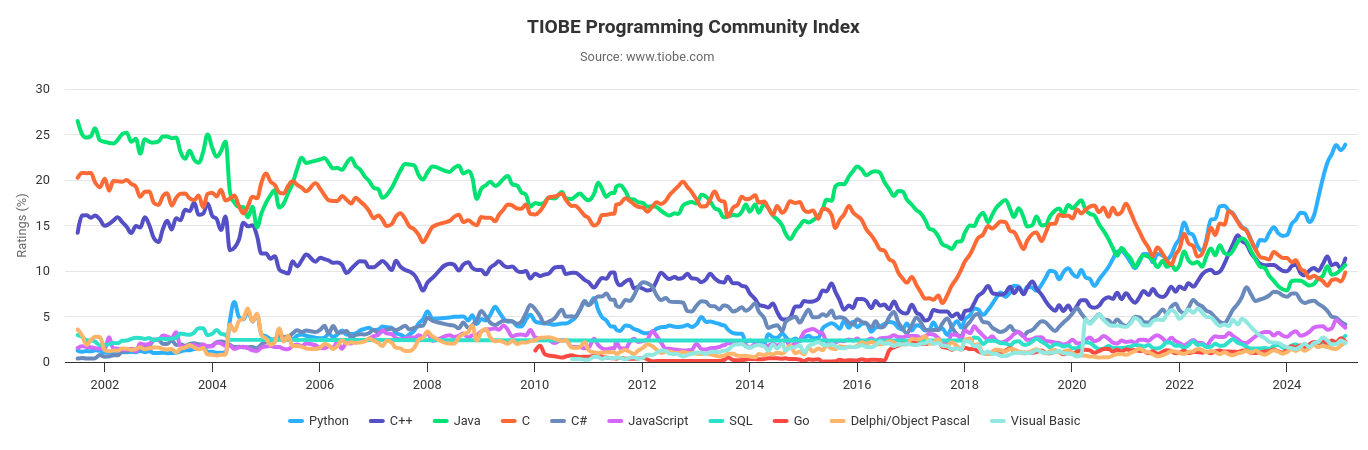
\includegraphics[width=0.8\textwidth]{pictures/Screenshot 2025-02-26 at 19-53-49 TIOBE Index - TIOBE}
        \caption{Entwicklung Tiobe Index 2002 - 2024 vom 26.02.2025 }
        \label{fig:entwicklung-tiobe}
    \end{figure}

    \begin{figure}[h]
        \centering
        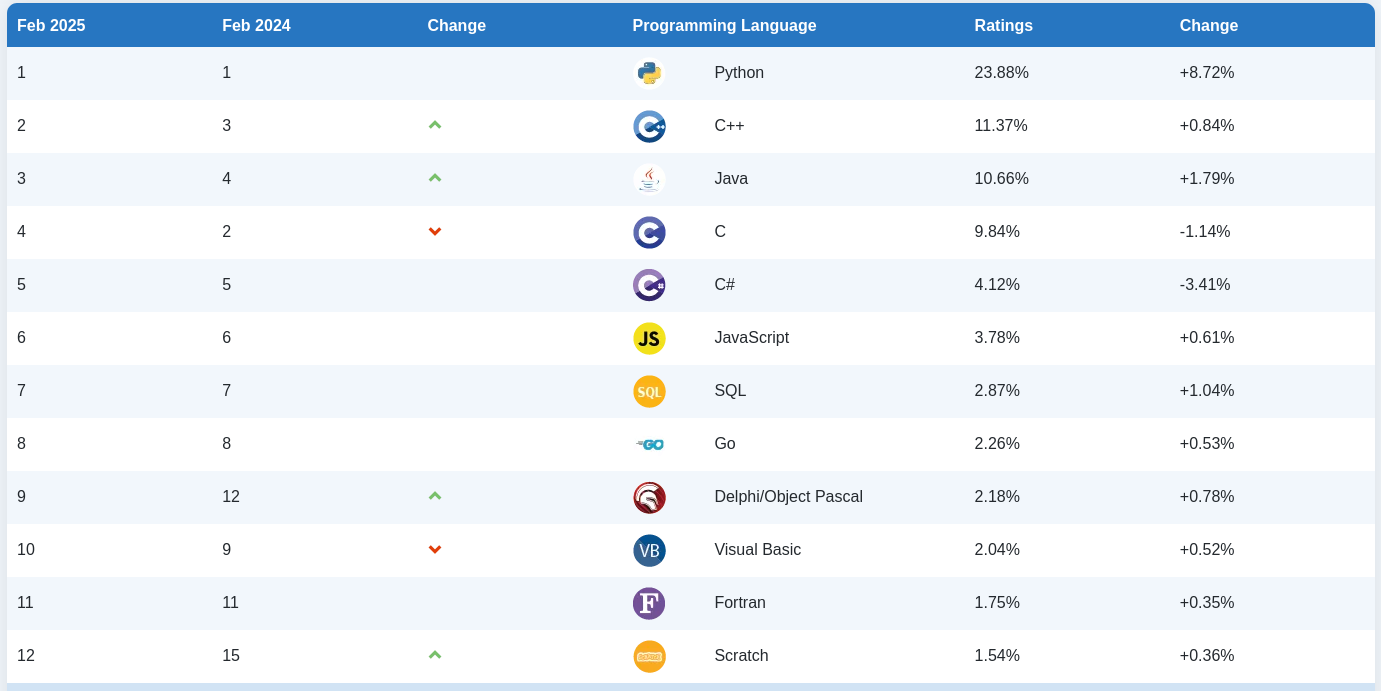
\includegraphics[width=0.8\textwidth]{pictures/Screenshot 2025-02-26 at 19-54-42 TIOBE Index - TIOBE}
        \caption{Tiobe Index Februar 2025 vom 26.02.2025}
        \label{fig:tiobe-java-2025}
    \end{figure}

    \begin{figure}[h]
        \centering
        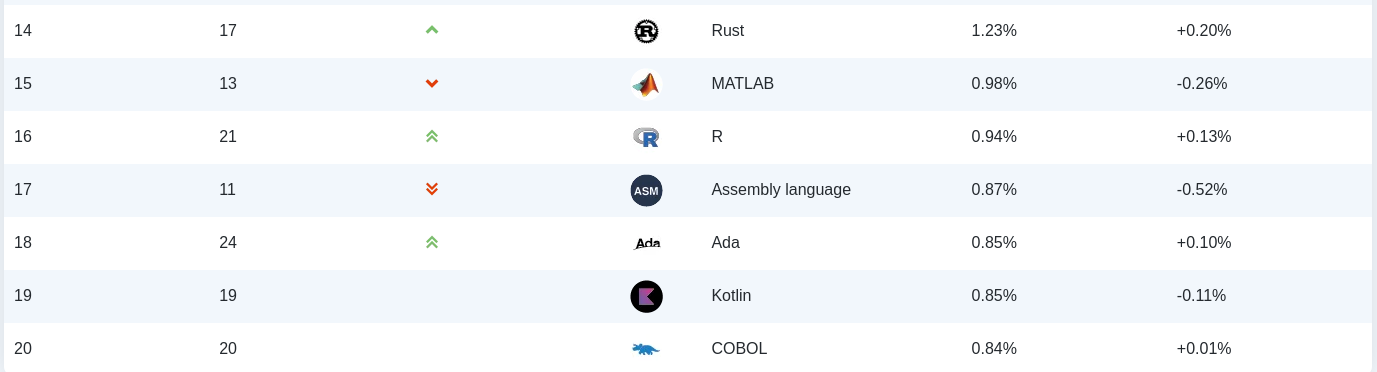
\includegraphics[width=0.8\textwidth]{pictures/Screenshot 2025-03-11 at 22-21-04 TIOBE Index - TIOBE}
        \caption{Tiobe Index März 2025 vom 11.03.2025}
        \label{fig:tiobe-kotlin-2025}
    \end{figure}


\end{document}